\documentclass{article}
\usepackage{amsmath}
\usepackage{url}
\bibliographystyle{apalike2}
\usepackage{natbib}
\usepackage{tikz}
\usepackage{hyperref}
\usepackage{mathtools}
\usepackage{enumitem}
\usepackage[a4paper, total={6in, 8in}]{geometry}
\usepackage{amssymb}
\usepackage{color}
\usepackage{lscape}
\usepackage{ifthen}
\usepackage{listings}
\usepackage{xcolor}
\usepackage{float}
\usepackage{booktabs}
\usepackage{hyperref}
\usepackage{fancyhdr}
\pagestyle{fancy}

\numberwithin{equation}{section}

% Define the header
\fancyfoot[L]{ECMA 31380 - Causal Machine Learning}
\fancyfoot[R]{Fernando Urbano}
\renewcommand{\footrulewidth}{0.2pt}
\fancyhead[L]{}
\fancyhead[C]{Comparative Analysis of DML Methods and DGPs for ATE Estimation in Diff. Causal Scenarios}
\fancyhead[R]{}

\usepackage{graphicx}
\setlength{\parskip}{0.5em}
\setlength{\parindent}{0pt}
\renewcommand{\thesubsection}{\thesection.\arabic{subsection}}
\newcommand{\divider}{\vspace{1em}\hrule\vspace{1em}}

\definecolor{codegreen}{rgb}{0, 0.6, 0}
\definecolor{codegray}{rgb}{0.5, 0.5, 0.5}
\definecolor{codepurple}{rgb}{0.58, 0, 0.82}
\definecolor{backcolour}{rgb}{0.95, 0.95, 0.92}
\newenvironment{colorparagraph}[1]{\par\color{#1}}{\par}
\definecolor{questioncolor}{RGB}{20, 40, 150}
\definecolor{annotationcolor}{RGB}{20, 200, 20}
\definecolor{tacolor}{RGB}{200, 0, 0}

\title{Comparative Analysis of Double Machine Learning Methods and Data Generating Processes for Average Treatment Effect Estimation in Diverse Causal Scenarios}
\author{Fernando Rocha Urbano}
\date{Autumn 2024}

\lstset{
    language=python,              
    basicstyle=\ttfamily\tiny,
    keywordstyle=\color{blue},    
    stringstyle=\color{red},      
    commentstyle=\color{gray},    
    showstringspaces=false,       
    numbers=left,                 
    numberstyle=\tiny\color{gray},
    stepnumber=1,                 
    breaklines=true,              
    frame=single,                 
    tabsize=4,                    
    captionpos=b,                 
    escapeinside={(*@}{@*)}       
}

\lstset{
    language=sql,                
    basicstyle=\ttfamily\tiny,
    keywordstyle=\color{blue},   
    stringstyle=\color{red},     
    commentstyle=\color{gray},   
    showstringspaces=false,      
    numbers=left,                
    numberstyle=\tiny\color{gray},
    stepnumber=1,                
    breaklines=true,             
    frame=single,                
    tabsize=4,                   
    captionpos=b,                
    escapeinside={(*@}{@*)}      
}

\newboolean{bool:showfrontdooradjustment}
\newboolean{bool:showquestions}
\newboolean{bool:showannotations}

\setboolean{bool:showfrontdooradjustment}{true}
\setboolean{bool:showquestions}{true}
\setboolean{bool:showannotations}{true}

\usetikzlibrary{arrows.meta, positioning}

\begin{document}

\maketitle

\section{Abstract}

This paper aims to establish and showcase theoretical background and practical implementation through simulations of data generating processes (DGPs) and the application of Double Machine Learning (DML) methods across various causal inference scenarios, including Backdoor Adjustment, Frontdoor Adjustment, and Instrumental Variables, especially in the context and goal of estimating the Average Treatment Effect (ATE).

We start by reviewing the literature and theoretical context of Double Machine Learning and dive into double robust estimation in the presence of instrumental variables, unobserved confounders, and mediators, showcasing differences in orthogonal score functions and implications of misspecification. We follow by reviewing the DGP under each of these causal scenarios, including the assumptions of each, the role of the nuisance functions in the estimation of the Average Treatment Effect (ATE), and the range of parameters that can be defined in simulations.

Finally, we develop a robust simulation framework capable of generating data under diverse causal settings, accommodating linear and nonlinear relationships, varying dimensions and sparsity of causal and non-causal covariates, and differing noise structures. The system serves as the building block of a long-term project that can evaluate the performance of DML methods in recovering the ATE across different causal scenarios.

We present a vast range of results for the Backdoor Adjustment scenario, exploring how various DML estimators perform in recovering the ATE. Here we provide actionable recommendations of which model between DNN, Random Forest, LASSO, Elastic Net, and OLS performs better under different conditions, highlighting differences in convergence rate, noise, nuisance function specification/misspecification, sample size, sparsity of covariates, and types of causal relationship between the target, treatment, and covariates (linear and non-linear).

\newpage
\tableofcontents
\newpage

\section{Double Machine Learning}

\subsection{Problem Setup}

Consider a random sample ${(Y_i, T_i, X_i)}_{i=1}^n$, where $Y_i \in \mathbb{R}$ is the outcome variable, $T_i \in \{0,1\}$ is a binary treatment indicator, and $X_i \in \mathbb{R}^d$ is a vector of covariates.

Our goal is to estimate the Average Treatment Effect (ATE), defined as:

\begin{equation}
\tau = \mathbb{E}[Y_i(1) - Y_i(0)],
\label{eq:tau_hat_potential_outcome}
\end{equation}

where $Y_i(t)$ denotes the potential outcome for unit $i$ under treatment $T_i = t$

The potential outcomes framework, introduced by \cite{Rubin1974} and continuously developed \cite{ImbensRubin2015}, conceptualizes the causal effect of a binary treatment \(T_i \in \{0,1\}\) on an outcome \(Y_i\) through the unobservable pair \((Y_i(0), Y_i(1))\).

In an ideal randomized experiment, the treatment assignment \(T_i\) is independent of these potential outcomes, ensuring unbiased estimates of the Average Treatment Effect (ATE). However, in observational data, the process that assigns treatment is rarely random, and \(T_i\) often depends on observed and possibly high-dimensional covariates \(X_i \in \mathbb{R}^d\).

This complicates the identification of the ATE, as one only observes \(Y_i(T_i)\) for each unit \(i\) while the counterfactual \(Y_i(1-T_i)\) remains unobserved. Thus, recovering the joint distribution of \((Y_i(0), Y_i(1))\) from the observed data \(\{(Y_i, T_i, X_i)\}_{i=1}^n\) is fundamentally a missing data problem.

In observational data, the Conditional Independence Assumption (CIA) is a crucial aspect of the potential outcomes framework, meaning that \((Y_i(0), Y_i(1)) \perp T_i \mid X_i\) must hold for us to correctly estimate the treatment effect. Under this assumption and overlap conditions ensuring \(0 < \mathbb{P}(T_i=1 \mid X_i) < 1\), one can express:

\begin{equation}
    \tau = \mathbb{E}[Y_i(1) - Y_i(0)] = \mathbb{E}[\mu_1(X_i) - \mu_0(X_i)],
\label{eq:tau_hat_potential_outcome_diff_means}
\end{equation}

where \(\mu_t(X_i) = \mathbb{E}[Y_i \mid T_i = t, X_i]\). Nonetheless, consistently estimating \(\mu_0(X)\), \(\mu_1(X)\), and thus \(\tau\) is challenging in practice.

First, any violations of CIA, including omitted confounders, wrong model specification, or measurement error in \(X_i\), will bias the estimates. Second, even if CIA holds, correct specification of the functional forms for \(\mu_0(X)\) and \(\mu_1(X)\) is difficult.

In modern settings, \(X_i\) is often high-dimensional, making parametric assumptions too restrictive and prone to model misspecification. Thus, an unbiased estimation of the ATE is often challenging \cite{Chernozhukov2018} and requires flexible, data-driven methods that can accommodate complex relationships between \(Y_i\), \(T_i\), and \(X_i\).

\subsection{From Linear Estimator to Double Robust Methods}
\label{subsec:from_linear_estimator_to_double_robust_methods}

Early approaches to estimating the ATE under the CIA often began with simple linear models for the outcome regression or propensity score. 

\begin{equation}
    \mu_t(X_i) = X_i^\top \beta_t \quad \text{and} \quad \pi(X_i) = X_i^\top \gamma,
\label{eq:linear_assumption_example}
\end{equation}

Such linear estimators assume that \(\mu_t(X_i)\) and \(\pi(X_i)=\mathbb{P}(T_i=1 \mid X_i)\) can be captured by low-dimensional linear functions of \(X_i\). However, any deviation from linearity or additivity, or the presence of omitted interactions, can result in substantial bias and inconsistent estimates of \(\tau\) \cite{ImbensRubin2015}.

To mitigate these issues, the literature has developed estimators that maintain consistency under weaker conditions. Chief among these are doubly robust estimators, which combine an outcome model and a propensity score model in such a way that if either one is correctly specified, the resulting ATE estimate remains consistent \cite{RobinsRotnitzkyZhao1994, BangRobins2005}. In other words, double robustness relaxes the strong reliance on fully correct functional specification of the data-generating process. This property becomes particularly appealing in high-dimensional settings, where even flexible parametric models may fail to capture all relevant nonlinearities and interactions \cite{Chernozhukov2018}.

By exploiting both an outcome regression model \(\mu_t(X_i)\) and a propensity score model \(\pi(X_i)\), doubly robust estimators attain unbiasedness under weaker conditions than either model alone would require. Specifically, if at least one of these models is correctly specified, the doubly robust estimator remains consistent for \(\tau\) \cite{RobinsRotnitzkyZhao1994, BangRobins2005}. A canonical example is the Augmented Inverse Probability Weighting (AIPW) estimator \cite{GlynnQuinn2010}:

\begin{equation}
    \hat{\tau}_{\text{DR}} = \frac{1}{n}\sum_{i=1}^n \left[
    \frac{T_i(Y_i - \hat{\mu}_1(X_i))}{\hat{\pi}(X_i)} + \hat{\mu}_1(X_i)
    - \frac{(1 - T_i)(Y_i - \hat{\mu}_0(X_i))}{1 - \hat{\pi}(X_i)} - \hat{\mu}_0(X_i)
    \right].
\label{eq:dr_estimator}
\end{equation}

In this construction, consistency does not hinge on both models being perfectly specified: correct specification of either \(\hat{\mu}_t(X_i)\) or \(\hat{\pi}(X_i)\) suffices to ensure unbiased estimation of \(\tau\).

While traditional doubly robust estimators often use parametric models for $\mu_t(X_i)$ and $\pi(X_i)$, DML explicitly incorporates machine learning techniques often able to capture complex relationships between $Y_i$, $T_i$, and $X_i$ without imposing strong parametric assumptions.

\subsection{DML Estimator}

The DML framework aims to estimate $\tau$ while controlling for high-dimensional or complex relationships between $Y_i$, $T_i$, and $X_i$. The key idea is to use machine learning methods to estimate the nuisance parameters and then construct an estimator for $\tau$ that is robust to estimation errors in these nuisance parameters.

\subsubsection{Nuisance Parameter Estimation}

We define the following nuisance functions:
\begin{align}
& m(X_i) = \mathbb{E}[Y_i | X_i],
\label{eq:m_x_for_target}
\\
& g(X_i) = \mathbb{E}[T_i | X_i],
\label{eq:g_x_for_treatment}
\\
& \pi(X_i) = \mathbb{P}(T_i = 1 | X_i) \quad \text{(propensity score)}
\label{eq:pi_x_for_treatment}
\end{align}

Such functions \(\{m(X_i), g(X_i), \pi(X_i)\}\) are called nuisance parameters because, while they characterize key components of the data-generating process, they are not directly of inferential interest for \(\tau\). Instead, they serve as building blocks that allow one to express the ATE through moment equations whose solutions return consistent and asymptotically normal estimators when these functions are known or well-estimated \cite{Chernozhukov2018, Newey1990, RobinsRotnitzkyZhao1994}.

In practice, \(\pi(X_i)\), the propensity score, controls for confounding by accounting for how units self-select into treatment based on their covariates. The functions \(m(X_i) = \mathbb{E}[Y_i \mid X_i]\) and \(g(X_i) = \mathbb{E}[T_i \mid X_i]\) capture the marginal relationships of the outcome and treatment with the covariates.

This property is achieved through Neyman-orthogonalization, ensuring that small perturbations in \(\hat{m}(X_i), \hat{g}(X_i), \hat{\pi}(X_i)\) do not accumulate into large biases in \(\hat{\tau}\) \cite{Chernozhukov2018, BelloniChernozhukovHansen2014}.

These functions can be estimated using flexible machine learning methods such as LASSO, Random Forests, or Neural Networks. Under mild regularity conditions and appropriate rates of convergence for the nuisance estimators, the DML estimator is root-n consistent and asymptotically normal (we make the regularity conditions explicity in Appendix~\ref{subsec:appendix_mild_regularity_conditions_for_dml}).

\subsubsection{Orthogonal Score Function}

To achieve robustness, we construct an orthogonal score function $\psi(Y_i, T_i, X_i; \eta)$, where $\eta = (m, g)$ represents the nuisance parameters. The orthogonal score satisfies the Neyman-orthogonality condition previously mentioned, which ensures that small estimation errors in $\eta$ have a negligible first-order impact on the estimation of $\tau$.

A common choice for the orthogonal score is for $T_i \in \{0,1\}$ and $Y_i \in \mathbb{R}$ is:
\begin{equation}
\psi(Y_i, T_i, X_i; \eta) = \left( \frac{T_i - g(X_i)}{\pi(X_i)(1 - \pi(X_i))} \right) (Y_i - m(X_i)) + \left( m_1(X_i) - m_0(X_i) \right) - \tau,
\label{eq:orthogonal_score}
\end{equation}

We derive the orthogonal score function in Section~\ref{subsec:appendix_orthogonal_score_function_backdoor_adjustment} (\cite{ChernozhukovChetverikovDemireretal2018}).

where $g(X_i) = \pi(X_i)$ and $m_t(X_i) = \mathbb{E}[Y_i | T_i = t, X_i]$ for $t \in \{0,1\}$.

\subsubsection{Estimation Procedure}

The estimation of DML models contains several steps:
\begin{enumerate}[label=\roman*.]
\item Estimate Nuisance Functions: Use one of the outlined ML models to obtain estimators $\hat{m}(X_i)$ and $\hat{g}(X_i)$ for the nuisance functions.

\item Compute the Score Function: Evaluate the orthogonal score $\psi(Y_i, T_i, X_i; \hat{\eta})$ using the estimated nuisance parameters.

\item Estimate $\tau$: Solve the empirical moment condition which yields $\hat{\tau}$:

\begin{equation}
\frac{1}{n} \sum_{i=1}^n \psi(Y_i, T_i, X_i; \hat{\eta}) = 0.
\label{eq:orthogonal_score_psi}
\end{equation}
\end{enumerate}

The orthogonal score function mitigates the impact of errors in $\hat{m}(X)$ and $\hat{g}(X)$ on the estimation of $\tau$ while also accomodating the use of modern ML techniques, allowing complex relationships between $Y$, $X$ and $T$.

To prevent overfitting while estimating the nuisance function and ensure that the estimation errors in the parameters do not bias the estimators of $\tau$, it is a common practice to employ cross-fitting.

\subsubsection{Cross-Fitting}

The steps of cross-fitting are:

\begin{enumerate}
\item Split the Sample: Divide the data into K folds $\{\mathcal{I}_k\}{k=1}^K$.
\item For Each Fold:
\begin{enumerate}
\item Train Nuisance Estimators: Use data from all other folds:
$$
\mathcal{I}_{-k} = \bigcup{j \neq k} \mathcal{I}_j
$$
to estimate $\hat{m}^{(-k)}(X_i)$ and $\hat{g}^{(-k)}(X_i)$.

\item Compute Score Function: For observations in fold $\mathcal{I}_k$, compute $\psi(Y_i, T_i, X_i; \hat{\eta}^{(-k)})$ using the nuisance estimates from step (a):

\begin{equation}
    \begin{split}
        \psi(Y_i, T_i, X_i; \hat{\eta}^{(-k)}) = & \left( \frac{T_i - \hat{g}^{(-k)}(X_i)}{\hat{\pi}^{(-k)}(X_i)} \right) (Y_i - \hat{m}^{(-k)}(X_i)) \\
        & + \ \hat{m}_1^{(-k)}(X_i) - \hat{m}_0^{(-k)}(X_i) - \tau^{(-k)}.
    \end{split}
    \label{eq:orthogonal_score_fold_k}
\end{equation}

\end{enumerate}
\item Aggregate: Combine the estimates from all folds:

\begin{equation}
\hat{\tau} = \frac{1}{n} \sum_{k=1}^K \sum_{i \in \mathcal{I}_k} \hat{\tau}_i^{(-k)} =  \frac{1}{K} \sum_{k=1}^K \hat{\tau}^{(-k)}
\label{eq:avg_tau_hat}
\end{equation}

\end{enumerate}

\section{Causal Inference Scenarios}

The three most relevant scenarios of causal inference are the ones that require Instrumental Variables, Backdoor Adjustment, or Front Door Adjustment.

To facilitate the understandig of the causal scenarios, we present the following notation, separating covariates in three different groups:
\begin{itemize}
    \item $C_i \in \mathbb{R}^{d_c}$: Confounders, variables that affect both the treatment $T_i$ and the outcome $Y_i$.
    \item $X_a \in \mathbb{R}^{d_a}$: Non-causal covariates, variables that do not affect the treatment $T_i$ or the outcome $Y_i$, but are correlated with the confounders $C_i$ and lead to misspecification when included in the model.
    \item $U_i \in \mathbb{R}^{d_u}$: Unobserved causal confounders, variables that affect both the treatment $T_i$ and the outcome $Y_i$ but are not observed. The non inclusion of $U_i$ in the model leads to misspecification and biased estimates of the causal effect unless a correction is present (IV scenario).
\end{itemize}

In the specified notation, CIA \eqref{subsec:from_linear_estimator_to_double_robust_methods} can be expressed as:

\begin{equation}
    Y_i(0), Y_i(1) \perp T_i \mid C_i, U_i
\end{equation}

A common way to represent the causal relation in the three scenarios previously mentioned is through the use of DAGs \cite{Pearl1995}.

\subsection{DAG (Directed Acyclic Graph)}

Directed Acyclic Graph (DAG) serves as a representation of causal assumptions and a tool for deriving statistical properties of the variables involved.

It is composed of nodes (vertices) representing random variables or features and directed edges (arrows), indicating a direct influence or causal effect (in \ref{fig:dag_example}, a causal effect of $T$ on $Y$).

\begin{figure}[H]
    \centering
    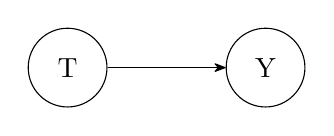
\begin{tikzpicture}[
        >={Stealth[round]},
        every node/.style={draw, circle, minimum size=1cm},
        every edge/.style={draw, ->, thick},
        node distance=2cm
    ]
    
    \node (T) {T};
    \node (Y) [right=of T, xshift=-0.5cm] {Y};
    
    \draw[->] (T) -- (Y);
    \end{tikzpicture}
    \caption{DAG Example}
    \label{fig:dag_example}
\end{figure}

The acyclic characterist is due to absence of directed cycles; that is, there is no path where you can start at a node $X$ and, by following directed edges, return to $X$.

\subsection{Backdoor Adjustment}

A backdoor path from treatment $T$ to the outcome $Y$ represents alternative routes through which association can flow from $T$ to $Y$ that are not due to the causal effect of $T$ on $Y$. In the representation, the confounder $C$ is a common cause of both $T$ and $Y$, thus, a backdoor path.

In such case, the association between $T$ and $Y$ may be partially or entirely due to their mutual dependence on $C$ rather than a direct causal effect, leading to biased causal estimates of the treatment if $C$ is ignored.

The causal effect of $T$ on $Y$ can be expressed using the backdoor adjustment formula:

\begin{equation}
    \mathbb{P}[Y(t)] = \sum_C \mathbb{P}[Y \mid T, C] \mathbb{P}[C],
\end{equation}

Which serves a markov factorization, calculating with respect to the DAG structure.

The scenario is the most commonly represented in causal inference, since it is present in most observational studies (where the treatment is not randomly assigned). It is often not even mentioned as a scenario, but as the standard case and already contains considerable part of its explanation in the previous sections.

For the backdoor adjustment to be valid, the following conditions must be satisfied:

\begin{enumerate}
    \item No variable in the adjustment set $C$ is a descendant of the treatment $T$.
    \item The adjustment set $C$ blocks all backdoor paths from $T$ to $Y$ (backdoor path is any path from $T$ to $Y$ that starts with an arrow into $T$).
\end{enumerate}

DAG~\ref{fig:dag_backdoor_path} illustrates the backdoor path involving the confounder $C$, treatment $T$, outcome $Y$, and features with non-causal association $X_a$ which would not be present in a typical backdoor adjustment DAG, but play a relevant role in the simulations proposed.

\begin{figure}[H]
    \centering
    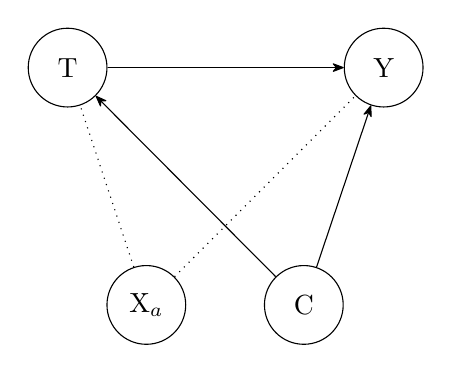
\begin{tikzpicture}[
        >={Stealth[round]},
        every node/.style={draw, circle, minimum size=1cm},
        every edge/.style={draw, ->, thick},
        node distance=2cm
    ]
    
    \node (T) {T};
    % \node (C) [above=of T, xshift=1.5cm] {C};
    \node (Y) [right=of T, xshift=1cm] {Y};
    \node (XC) [below=of T, xshift=3cm] {$\text{C}$};
    \node (XA) [below=of T, xshift=1cm] {$\text{X}_a$};
    
    % \draw[->] (C) -- (T);
    % \draw[->] (C) -- (Y);
    \draw[->] (T) -- (Y);  
    \draw[->] (XC) -- (T);
    \draw[->] (XC) -- (Y);
    \draw[dotted] (XA) -- (T);
    \draw[dotted] (XA) -- (Y);
    \end{tikzpicture}
    \caption{DAG of Backdoor Path}
    \label{fig:dag_backdoor_path}
\end{figure}

\subsubsection{Backdoor Adjustment Scenario in DML}

In Backdoor Adjustment with DML, the ideal $m(X_i) = \mathbb{E}[Y_i | X_i]$ and $g(X_i) = \mathbb{E}[T_i | X_i]$ from Equations \eqref{eq:m_x_for_target} and \eqref{eq:g_x_for_treatment} are:

\begin{align}
    & m_{\text{BA}}(C_i) = \mathbb{E}[Y_i | C_i],
    \label{eq:m_x_for_target_backdoor_adjustment}
    \\
    & g_{\text{BA}}(C_i) = \mathbb{E}[T_i | C_i],
    \label{eq:g_x_for_treatment_backdoor_adjustment}
\end{align}

In our simulations we also test the habilit of the ML models to estimate ATE under the following scenarios. In these scenarios, the superscript $\text{w}_i$ on the nuisance functions denotes the i-th scenario which involves misspecifications of the nuisance functions.

\paragraph{Inclusion of $C_i$ and $X_{a, i}$ on every nuisance function}

\begin{align}
    & m_{\text{BA}}^{\text{w}_1}(C_i, X_{a, i}) = \mathbb{E}[Y_i | C_i, X_{a, i}],
    \label{eq:m_x_for_target_backdoor_adjustment_wrong_1}
    \\
    & g_{\text{BA}}^{\text{w}_1}(C_i, X_{a, i}) = \mathbb{E}[T_i | C_i, X_{a, i}],
    \label{eq:g_x_for_treatment_backdoor_adjustment_wrong_1}
\end{align}

Equations \eqref{eq:m_x_for_target_backdoor_adjustment_wrong_1} and \eqref{eq:g_x_for_treatment_backdoor_adjustment_wrong_1} represent a scenario in which one would not be aware that $X_a$ does not cause $T$ and $Y$.

\paragraph{Only partial inclusion of $C_i$ and inclusion of $X_{a, i}$ on every nuisance function}
\label{par:backdoor_adjustment_wrong_2}

\begin{align}
    & m_{\text{BA}}^{\text{w}_2}(C^{p}_i, X_{a, i}) = \mathbb{E}[Y_i | C^{p}_i, X_{a, i}],
    \label{eq:m_x_for_target_backdoor_adjustment_wrong_2}
    \\
    & g_{\text{BA}}^{\text{w}_2}(C^{p}_i, X_{a, i}) = \mathbb{E}[T_i | C^{p}_i, X_{a, i}],
    \label{eq:g_x_for_treatment_backdoor_adjustment_wrong_2}
\end{align}

Equations \eqref{eq:m_x_for_target_backdoor_adjustment_wrong_2} and \eqref{eq:g_x_for_treatment_backdoor_adjustment_wrong_2} also represent a scenario in which one would not be aware that $X_a$ does not cause $T$ and $Y$ and also does not include all causal cofounders. $C^{p}_i$ is subset of $C_i$ included, where $C_i \in \mathbb{R}^{d_c}$ and $C^{p}_i \in \mathbb{R}^{d_{cp}}$ and $d_c > d_{cp}$.

\subsection{Frontdoor Adjustment}

Frontdoor adjustment is a method used to estimate the causal effect of treatment $T$ on outcome $Y$ when there is unmeasured confounding that cannot be addressed using backdoor adjustment. It leverages a mediator $M$ that lies on the causal path from $T$ to $Y$.

The causal effect of $T$ on $Y$ can be expressed using the frontdoor adjustment formula:

\begin{equation}
\mathbb{P}[Y(t)] = \sum_M \mathbb{P}[M \mid T=t] \sum_{t’} \mathbb{P}[Y \mid M, T=t’] \mathbb{P}[T=t’].
\end{equation}

$t'$ acts as a dummy variable of integration (or summation) which, in our case, assumes values in $\{0, 1\}$. The $\mathbb{P}[Y(t)]$ is computed by marginalizing over both the mediator $M$ and any variation in the treatment $T$ \cite{Pearl2012}

For instance, the average treatment effect in case $M, T \in \{0, 1\}$:

\begin{equation}
\tau = \left[ \mathbb{P}(M = 1 \mid T = 1) - \mathbb{P}(M = 1 \mid T = 0) \right] \times \left[ \mathbb{E}[Y \mid M = 1] - \mathbb{E}[Y \mid M = 0] \right]
\end{equation}

For the frontdoor adjustment to be valid, the following conditions must be satisfied:

\begin{enumerate}
\item All causal paths from $T$ to $Y$ pass through $M$ (i.e., there is no direct effect of $T$ on $Y$ bypassing $M$).
\item There are no unmeasured confounders between $T$ and $M$.
\item All backdoor paths from $M$ to $Y$ are blocked by $T$ (i.e., there are no unmeasured confounders between $M$ and $Y$ that are not affected by $T$).
\end{enumerate}

DAG~\ref{fig:dag_frontdoor_path} illustrates the frontdoor adjustment involving the treatment $T$, mediator $M$, outcome $Y$, observed confounders $C$ and features with no causal association $X_a$. $C$ and $X_a$ would not be present in a typical frontdoor adjustment DAG, but are included due to their relevance in the proposed simulations.

\begin{figure}[H]
    \centering
    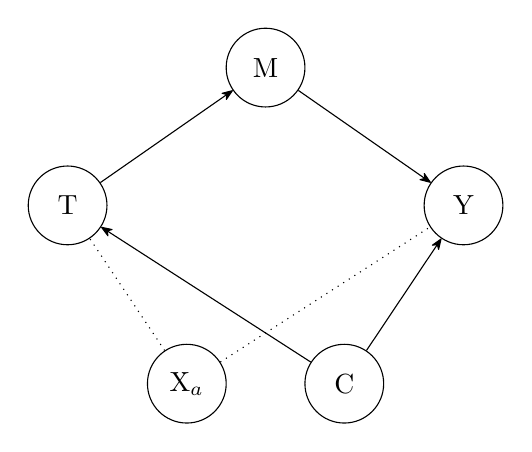
\begin{tikzpicture}[
        >={Stealth[round]},
        every node/.style={draw, circle, minimum size=1cm},
        every edge/.style={draw, ->, thick},
        node distance=2cm
    ]
    
    \node (T) {T};
    \node (M) [right=of T, xshift=-0.5cm, yshift=1.75cm] {M};
    \node (Y) [right=of M, xshift=-0.5cm, yshift=-1.75cm] {Y};
    \node (XA) [below=of M, xshift=-1cm, yshift=-1cm] {$\text{X}_a$};
    \node (XC) [below=of M, xshift=1cm, yshift=-1cm] {C};
    
    \draw[->] (T) -- (M);
    \draw[->] (M) -- (Y);
    \draw[->] (XC) -- (T);
    \draw[->] (XC) -- (Y);
    \draw[dotted] (XA) -- (T);
    \draw[dotted] (XA) -- (Y);
    \end{tikzpicture}
    \caption{DAG of Frontdoor Path}
    \label{fig:dag_frontdoor_path}
\end{figure}

\subsubsection{Frontdoor Adjustment Scenario in DML}

In our simulations, we use a binary mediator $M_i \in \{0, 1\}$, similar to the binary treatment $T_i$.

In the Frontdoor Adjustment scenario with DML, we need to account for the mediator $M_i$ when estimating the ATE. The identification of the causal effect involves modeling the relationships between $T_i$, $M_i$, and $Y_i$.

The ideal nuisance functions for DML in this scenario are:

\begin{align}
    & m_{\text{FA}}(M_i, C_i) = \mathbb{E}[Y_i \mid M_i, C_i],
    \label{eq:m_x_for_target_frontdoor_adjustment} \\
    & h_{\text{FA}}(T_i) = \mathbb{E}(M_i \mid T_i),
    \label{eq:h_x_for_mediator_frontdoor_adjustment} \\
    & g_{\text{FA}}(C_i) = \mathbb{E}(T_i \mid C_i),
    \label{eq:g_x_for_treatment_frontdoor_adjustment}
\end{align}

Here $h_{\text{FA}}(M_i, T_i, C_i)$ is the mediator model, representing the probability of the mediator given treatment.

To adapt the orthogonal score function in the presence of the mediator, we modify Equation~\eqref{eq:orthogonal_score} to incorporate the mediator's effect ((\cite{ChernozhukovChetverikovDemireretal2018})). The adapted orthogonal score function is:

\begin{equation}
    \begin{split}
        \psi(Y_i, T_i, M_i, C_i; \eta) = \\ \left(
        \left(
            \frac{M_i - h_{\text{FA}}(T_i)}{h_{\text{FA}}(T_i)(1 - h_{\text{FA}}(T_i))}
        \right) (Y_i - m_{\text{FA}}(M_i, C_i))
        \right)
        \cdot \left(
            h_{\text{FA}}(T_i = 1) - h_{\text{FA}}(T_i = 0)
        \right)
        - \tau
    \end{split}
    \label{eq:orthogonal_score_frontdoor}
\end{equation}

In this score function:

\begin{itemize}
    \item The first term adjusts for the probability of the mediator and its interaction with the outcome.
    \item The second term adjusts for the probability of the mediator given treatment.
\end{itemize}

We derive the orthogonal score function for Frontdoor Adjustment in Section~\ref{subsec:appendix_orthogonal_score_function_frontdoor_adjustment}.

In our simulations we also test the hability of the ML models to estimate ATE under the following scenario.

\paragraph{Inclusion of $C_i$ and $X_{a, i}$ on every nuisance function}

\begin{align}
    & m_{\text{FA}}^{\text{w}_1}(M_i, C_i, X_{a, i}) = \mathbb{E}[Y_i \mid M_i, C_i, X_{a, i}],
    \label{eq:m_x_for_target_frontdoor_adjustment_wrong_1} \\
    & h_{\text{FA}}^{\text{w}_1}(T_i, C_i, X_{a, i}) = \mathbb{E}(M_i \mid C_i, X_{a, i}),
    \label{eq:h_x_for_mediator_frontdoor_adjustment_wrong_1} \\
    & g_{\text{FA}}^{\text{w}_1}(C_i, X_{a, i}) = \mathbb{E}(T_i \mid C_i, X_{a, i}),
    \label{eq:g_x_for_treatment_frontdoor_adjustment_wrong_1}
\end{align}

Equations \eqref{eq:m_x_for_target_frontdoor_adjustment_wrong_1}, \eqref{eq:h_x_for_mediator_frontdoor_adjustment_wrong_1}, and \eqref{eq:g_x_for_treatment_frontdoor_adjustment_wrong_1} represent a scenario where one is unaware that $X_{a, i}$ has no causal relation to $T_i$, $M_i$, or $Y_i$. Equation \eqref{eq:h_x_for_mediator_frontdoor_adjustment_wrong_1} represents scenarion where one is unaware that $C$ has no causal relation to $M_i$.

\paragraph{Ignoring the mediator $M_i$}

\begin{align}
    & m_{\text{FA}}^{\text{w}_2}(C_i, X_{a, i}) = \mathbb{E}[Y_i \mid C_i, X_{a, i}],
    \label{eq:m_x_for_target_frontdoor_adjustment_wrong_2} \\
    & g_{\text{FA}}^{\text{w}_2}(C_i, X_{a, i}) = \mathbb{E}[T_i \mid C_i, X_{a, i}],
    \label{eq:g_x_for_treatment_frontdoor_adjustment_wrong_2}
\end{align}

Equations \eqref{eq:m_x_for_target_frontdoor_adjustment_wrong_2} and \eqref{eq:g_x_for_treatment_frontdoor_adjustment_wrong_2} represent a scenario where the mediator $M_i$ is unavailable or ignored and one is unaware that $X_{a, i}$ has no causal relationship to $T$ or $Y$. In this case, the orthogonal score function is the same as in Equation~\eqref{eq:orthogonal_score}.

\paragraph{Considering the mediator $M_i$ as a normal covariate}

\begin{align}
    & m_{\text{FA}}^{\text{w}_3}(C_i, M_i, X_{a, i}) = \mathbb{E}[Y_i \mid C_i, M_i, X_{a, i}],
    \label{eq:m_x_for_target_frontdoor_adjustment_wrong_3} \\
    & g_{\text{FA}}^{\text{w}_3}(C_i, M_i, X_{a, i}) = \mathbb{E}[T_i \mid C_i, M_i, X_{a, i}],
    \label{eq:g_x_for_treatment_frontdoor_adjustment_wrong_3}
\end{align}

Equations \eqref{eq:m_x_for_target_frontdoor_adjustment_wrong_3} to \eqref{eq:g_x_for_treatment_frontdoor_adjustment_wrong_3} also represent scenarios where one is unaware that $X_{a, i}$ has no causal relation to $T_i$ or $Y_i$, and the scenario where $M_i$ is available but not recognized as a mediator. In this case, the orthogonal score function is the same as in Equation~\eqref{eq:orthogonal_score}.

\subsection{Instrumental Variable}

Instrumental variable (IV) estimation is a method used to estimate the causal effect of a treatment $T_i$ on an outcome $Y_i$ when there is unmeasured confounding $U_i$ that cannot be addressed using backdoor or frontdoor adjustments. This method leverages an instrument $Z_i$, which influences the treatment $T_i$ but has no direct effect on the outcome $Y_i$  except through $T_i$, and is independent of any unmeasured confounders $U_i$ affecting both $T_i$ and $Y_i$.

For the instrumental variable method to be valid, the following conditions must be satisfied:

\begin{enumerate}
\item Relevance: The instrument $Z$ is associated with the treatment  $T$  (i.e.,  $\text{Cov}(Z, T) \neq 0$  or \( Z \not\!\perp\!\!\!\perp T \)).
\item Exclusion Restriction: The instrument $Z$ affects the outcome $Y$ only through its effect on the treatment $T$ (i.e., there is no direct effect of $Z$ on $Y$ and no other pathways from $Z$ to $Y$ except through  $T$).
\item Independence (Ignorability): The instrument $Z$ is independent of any unmeasured confounders $U$ that affect both $T$ and $Y$ $(i.e.,  Z \perp\!\!\!\perp U )$.
\end{enumerate}

DAG~\ref{fig:dag_instrumental_variable} illustrates the instrumental variable setup involving the unobserved confounder $U$, instrument $Z$, treatment $T$, outcome $Y$, observed confounder $C$, and features with non-causal associations $X_a$. Again, the last two would not be present in a typical instrumental variable DAG, but are included due to their relevance in the proposed simulations.

\begin{figure}[H]
    \centering
    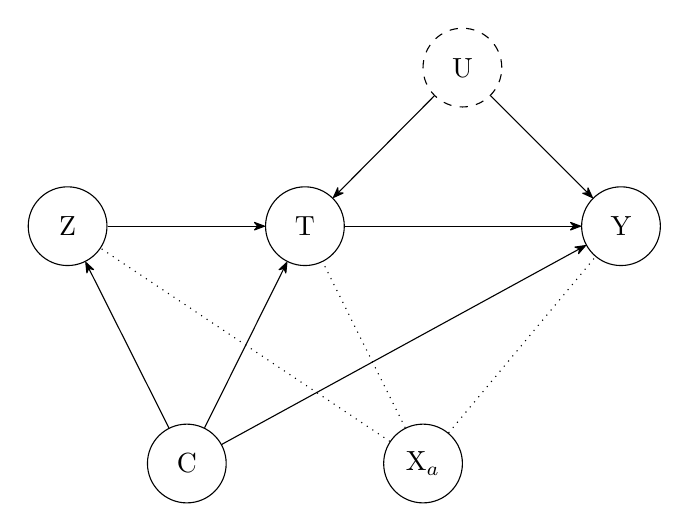
\begin{tikzpicture}[
        >={Stealth[round]},
        every node/.style={draw, circle, minimum size=1cm},
        every edge/.style={draw, ->, thick},
        node distance=2cm
    ]
    
    \node (Z) {Z};
    \node (T) [right=of Z] {T};
    \node (U) [above=of T, xshift=2cm, yshift=-1cm, dashed] {U};
    \node (XC) [below=of T, xshift=-1.5cm] {$\text{C}$};
    \node (XA) [below=of T, xshift=1.5cm] {$\text{X}_a$};
    \node (Y) [right=of T, xshift=1cm] {Y};
    
    \draw[->] (Z) -- (T);
    \draw[->] (T) -- (Y);
    \draw[->] (U) -- (T);
    \draw[->] (U) -- (Y);
    \draw[->] (XC) -- (T);
    \draw[->] (XC) -- (Z);
    \draw[->] (XC) -- (Y);
    \draw[dotted] (XA) -- (T);
    \draw[dotted] (XA) -- (Z);
    \draw[dotted] (XA) -- (Y);
    \end{tikzpicture}
    \caption{DAG of Instrumental Variable}
    \label{fig:dag_instrumental_variable}
\end{figure}
    
\subsubsection{Instrumental Variable Scenario in DML}

To adapt the DML framework to the IV setting, we need to define appropriate nuisance functions and construct an orthogonal score function suitable for the IV context.

The ideal nuisance functions in this scenario are:

\begin{align}
    & m_{\text{IV}}(C_i) = \mathbb{E}[Y_i \mid C_i],
    \label{eq:m_x_for_target_instrumental_variable} \\
    & q_{\text{IV}}(C_i) = \mathbb{E}[Z_i \mid C_i],
    \label{eq:q_z_for_instrument_instrumental_variable} \\
    & g_{\text{IV}}(C_i) = \mathbb{E}[T_i \mid C_i],
    \label{eq:g_x_for_treatment_instrumental_variable}
\end{align}

Where $m_{\text{IV}}(C_i)$ is the outcome model, capturing the expected outcome given covariates, $q_{\text{IV}}(C_i)$ is the instrument propensity score, representing the expected treatment given the instrument and covariates, and $g_{\text{IV}}(C_i)$ is the treatment model, representing the expected treatment given covariates.

The orthogonal score function for the IV scenario is different from the standard DML orthogonal score function (\cite{BelloniChernozhukovHansen2014, ChernozhukovChetverikovDemireretal2018}). An appropriate orthogonal score function in the linear IV context is:

\begin{equation}
    \psi(Y_i, T_i, Z_i, C_i; \tau, \eta) = \left( Y_i - m_{\text{IV}}(C_i) - \tau [T_i - g_{\text{IV}}(C_i)] \right) \left( Z_i - q_{\text{IV}}(C_i) \right),
    \label{eq:orthogonal_score_iv}
\end{equation}

We derive the orthogonal score function for Frontdoor Adjustment in Section~\ref{subsec:appendix_orthogonal_score_function_instrumental_variable}.

In our simulations we also test the habilit of the ML models to estimate ATE under the following scenarios. In these scenarios, the superscript $\text{w}_i$ on the nuisance functions denotes the i-th scenario which involves misspecifications of the nuisance functions.

\paragraph{Inclusion of $C_i$ and $X_{a, i}$ on every nuisance function}

\begin{align}
    & m_{\text{IV}}^{\text{w}_1}(C_i) = \mathbb{E}[Y_i \mid C_i, X_{a, i}],
    \label{eq:m_x_for_target_instrumental_variable_wrong_1} \\
    & q_{\text{IV}}^{\text{w}_1}(C_i) = \mathbb{E}[Z_i \mid C_i, X_{a, i}],
    \label{eq:q_z_for_instrument_instrumental_variable_wrong_1} \\
    & g_{\text{IV}}^{\text{w}_1}(C_i) = \mathbb{E}[T_i \mid C_i, X_{a, i}],
    \label{eq:g_x_for_treatment_instrumental_variable_wrong_1}
\end{align}

Equations \eqref{eq:m_x_for_target_instrumental_variable_wrong_1}, \eqref{eq:q_z_for_instrument_instrumental_variable_wrong_1}, and \eqref{eq:g_x_for_treatment_instrumental_variable_wrong_1} represent a scenario in which one would not be aware that $X_a$ does not cause $T$, $Z$ and $Y$.

\paragraph{Only partial inclusion of $C_i$ and inclusion of $X_{a, i}$ on every nuisance function}

\begin{align}
    & m_{\text{IV}}^{\text{w}_2}(C_i^{p}, X_{a, i}) = \mathbb{E}[Y_i \mid C_i, X_{a, i}],
    \label{eq:m_x_for_target_instrumental_variable_wrong_2} \\
    & q_{\text{IV}}^{\text{w}_2}(C_i^{p}, X_{a, i}) = \mathbb{E}[Z_i \mid, C_i, X_{a, i}],
    \label{eq:q_z_for_instrument_instrumental_variable_wrong_2} \\
    & g_{\text{IV}}^{\text{w}_2}(C_i^{p}, X_{a, i}) = \mathbb{E}[T_i \mid C_i, X_{a, i}],
    \label{eq:g_x_for_treatment_instrumental_variable_wrong_2}
\end{align}

Equations \eqref{eq:m_x_for_target_instrumental_variable_wrong_2}, \eqref{eq:q_z_for_instrument_instrumental_variable_wrong_2}, and \eqref{eq:g_x_for_treatment_backdoor_adjustment_wrong_2} also represent a scenario in which one would not be aware that $X_a$ does not cause $T$ and $Y$ and also does not include all causal cofounders. $C^{p}_i$ is subset of $C_i$ included, where $C_i \in \mathbb{R}^{d_c}$ and $C^{p}_i \in \mathbb{R}^{d_{cp}}$ and $d_c > d_{cp}$.

\paragraph{$Z_i$ is treated as a normal cofounder}

\begin{align}
    & m_{\text{IV}}^{\text{w}_3}(C_i, Z_i) = \mathbb{E}[Y_i | C_i, Z_i],
    \label{eq:m_x_for_target_instrumental_variable_wrong_3}
    \\
    & g_{\text{IV}}^{\text{w}_3}(C_i, Z_i) = \mathbb{E}[T_i | C_i, Z_i],
    \label{eq:g_x_for_treatment_instrumental_variable_wrong_3}
\end{align}

Equations \eqref{eq:m_x_for_target_instrumental_variable_wrong_3} and \eqref{eq:g_x_for_treatment_instrumental_variable_wrong_3} represent a scenario in which one would treat $Z$ as a normal covariate. In this case, the orthogonal score function would be the same as in the backdoor adjustment scenario of \eqref{eq:orthogonal_score}.

\paragraph{$Z_i$ is treated as a normal cofounder and inclusion of $X_{a, i}$ on every nuisance function}

\begin{align}
    & m_{\text{IV}}^{\text{w}_4}(C_i, Z_i, X_{a, i}) = \mathbb{E}[Y_i | C_i, Z_i, X_{a, i}],
    \label{eq:m_x_for_target_instrumental_variable_wrong_3}
    \\
    & g_{\text{IV}}^{\text{w}_4}(C_i, Z_i, X_{a, i}) = \mathbb{E}[T_i | C_i, Z_i, X_{a, i}],
    \label{eq:g_x_for_treatment_instrumental_variable_wrong_3}
\end{align}

Equations \eqref{eq:m_x_for_target_instrumental_variable_wrong_3} and \eqref{eq:g_x_for_treatment_instrumental_variable_wrong_3} represent a scenario in which one would treat $Z$ as a normal covariate and is not aware that $X_a$ does not cause $T$, $Z$ and $Y$. In this case, the orthogonal score function would also be the same as in the backdoor adjustment scenario of \eqref{eq:orthogonal_score}.

\section{Simulation Methodology}

\subsection{Data Generating Process}

We define the the backdoor path scenario as the typical scenario. The frontdoor path and instrumental variable scenarios are variations of the typical scenario.

\subsubsection{Cofounders}

The cofounders are generated with multivariate normal distribution using a sparse covariance matrix $\Sigma_d$ and a vector of means $\boldsymbol{\mu}_d = \bf{0}$.

$\Sigma_d \in \mathbb{R}^{d \times d}$, where $d := d_a + d_c$. $d_a$ is the number of non-causal confounders previously represented as $X_a$ and $d_c$ is the number of causal confounders previously represented as $C$.

\begin{equation}
    \label{eq:cofounders_data_generating_process}
    X \sim \mathcal{N}_d(\boldsymbol{\mu}_d, \Sigma_d)
\end{equation}

The sparsity of the covariance matrix of the cofounders $\Sigma_d$ is determined by $\alpha_d$, which represents the probability that any covariance coefficient is zero. Larger $\alpha_d$'s result in sparser covariance matrices. To provide intuition on it, we report the average absolute correlation ${|\rho_d|}$ in the matrix.

After generating the data from the multivariate normal distribution defined as $X \in \mathbb{R}^{n \times d}$ we randomly separate the features of $X$ in $X_a$ and $C$. Following the logic specified above, $X_a \in \mathbb{R}^{n \times d_a}$ and $C \in \mathbb{R}^{n \times d_c}$.

In \eqref{eq:m_x_for_target_backdoor_adjustment_wrong_2} and \eqref{eq:g_x_for_treatment_backdoor_adjustment_wrong_2} ``Only partial inclusion of $C_i$ and inclusion of $X_{a, i}$ on every nuisance function'', after generating cofounders, treatment, and target, we select a subset of the causal confounders $C^{p}_i$ to be used in the nuisance functions. This would represent a scenario of unobserved confounders $U_i$. We define which causal confounders are not included in the nuisance function randomly, through the use of $p_u$, which represents the percentage of causal confounders not included in the nuisance functions. Meaning that $C^{p}_i \in \mathbb{R}^{n \times d_{cp}}$, where $d_{cp} = d_c - \lceil p_u \cdot d_c \rceil$.

\subsubsection{Treatment}

The probability of treatment is generated from a logic:

\begin{equation}
    \mathbb{P}[T_i] = \frac{1}{1 + e^{(-f(C_i) + \varepsilon_{t, i})}}
    \label{eq:probability_of_treatment}
\end{equation}

where $f(C_i)$ is a function of the causal confounders $C_i$ and $\varepsilon_{t, i}$ is a random error term generated from a normal distribution with mean 0 and variance $\sigma_{t}$.

$f(C_i)$ is a generic non-linear function explained in Section~\ref{subsubsec:f_c_non_linear_relationship}.

Treatment is later generated from a Bernoulli distribution with the probability of treatment from above in \eqref{eq:probability_of_treatment}.

\begin{equation}
    T_i \sim Bernoulli(\mathbb{P}[T_i])
\end{equation}

\subsubsection{Treatment Effect}

The true individual treatment effect is generated from:

\begin{equation}
    \tau_i(C_i) = f(C_i)
    \label{eq:treatment_effect}
\end{equation}

Again, $f(C_i)$ is a generic non-linear function explained in Section~\ref{subsubsec:f_c_non_linear_relationship}.

Meaning that there is heterogeneity in the treatment effect across the causal confounders $C_i$.

The true ATE (Average Treatment Effect) is the average of the treatment effect across the population:

\begin{equation}
    \tau = \mathbb{E}[\tau(C_i)] = \frac{1}{n} \sum_{i=1}^{n} \tau_i(C_i)
\end{equation}

\subsubsection{Outcome}

The observed outcome for each individual is:

\begin{equation}
    Y_i = Y_{i, 0} + \tau_i(C_i) \cdot T_i + \varepsilon_{y, i}, \quad \varepsilon_{y, i} \sim \mathcal{N}(0, \sigma_{y})
    \label{eq:observed_outcome}
\end{equation}

where $Y_{i, 0}$ is the potential outcome if the treatment $T_i$ was not applied, $\tau_i(C_i)$ is the treatment effect, and $\varepsilon_{y, i}$ is a random error term generated from a normal distribution with mean 0 and variance $\sigma_{y}$.

\begin{equation}
    Y_{i, 0} = f(C_i)
    \label{eq:potential_outcome_no_treatment}
\end{equation}

Once more, $f(C_i)$ is a generic non-linear function explained in Section~\ref{subsubsec:f_c_non_linear_relationship}.

The potential outcome for treatment and control are:

\begin{equation}
    Y_i(1) = Y_{i, 0} + \tau_i(C_i), \quad Y_i(0) = Y_{i, 0},
    \label{eq:potential_outcomes}
\end{equation}

which can not be directly observed.

\subsubsection{$f(C_i)$ Non-Linear Transformation}
\label{subsubsec:f_c_non_linear_relationship}

The function $f(C_i)$, used to calculate $Y_{i, 0}$ and $\mathbb{P}[T_i]$ is a generic function composed non-linear relationships.

More specifically $f(C_i)$ is the weighted sum of of different ``$q$'' transformations in the causal confounders $C_i$:

\begin{equation}
    f(C) = \sum_{j=1}^{d_c} \left( \beta_{j} \cdot q_j(C_{j}) \right)
\end{equation}

Where $C_{j}$ is the the vector of the $j$-th causal confounder, $\beta_j$ is a random coefficient drawn from a uniform distribution $U(-1, 1)$, and $q_j(C_{j})$ is a random transformation of the $j$-th causal confounder. More specifically, the chosen transformation $q_j(C_{j})$ is randomly chosen from the following set of possible transformations:

\begin{figure}[H]
\begin{enumerate}[label=\roman*.]
    \item Linear: $q_j(C_{i, j}) = C_{i, j}$
    \item Quadratic: $q_j(C_{i, j}) = C_{i, j}^2$
    \item Cubic: $q_j(C_{i, j}) = C_{i, j}^3$
    \item Logarithmic: $q_j(C_{i, j}) = \log(|C_{i, j}| + 1)$
    \item Exponential: $q_j(C_{i, j}) = \exp(\frac{1}{5} C_{i, j})$
    \item Sine: $q_j(C_{i, j}) = \sin(C_{i, j})$
    \item Cosine: $q_j(C_{i, j}) = \cos(C_{i, j})$
    \item Indicator: $q_j(C_{i, j}) = \mathbb{I}\{C_{i, j} > 0\} - \mathbb{I}\{C_{i, j} \leq 0\}$
    \item Piecewise: $q_j(C_{i, j}) = 2 \mathbb{I}\{C_{i, j} < 0\} + \mathbb{I}\{0 \leq C_{i, j} < 1\} + \frac{1}{2} \mathbb{I}\{ C_{i, j} > 1\}$
\end{enumerate}
\end{figure}

For each simulation, $f(C)$ is calculated with some of the specified transformation sets and $\beta$'s three times: one for the calculation of $Y_{i, 0}$, one for the calculation of $\mathbb{P}[T_i]$, and one for the calculation of $\tau_i(C_i)$.

For some simulations, we only allow for linear transformations in $f(C)$, aiming to compare performance of the DML models in a simpler setting.

\subsubsection{Parameter Tuning in the Data Generating Process}
\label{subsubsec:parameter_tuning_in_the_data_generating_process_backdoor}

The data generating process has some parameters that can be tuned to generate different scenarios. We present the following variations:

\begin{enumerate}[label=\roman*.]
    \item $f(C_i)$ for Treatment Probability: linear or non-linear transformations \eqref{eq:probability_of_treatment}.
    \item $f(C_i)$ for Treatment Effect: linear or non-linear transformations \eqref{eq:treatment_effect}.
    \item $f(C_i)$ for Outcome: linear or non-linear transformations \eqref{eq:potential_outcome_no_treatment}.
    \item $d_c$: number of causal confounders.
    \item $d_a$: number of non-causal confounders.
    \item $p_u$: percentage of causal confounders not included in the nuisance functions in the backdoor adjustment scenario with wrong specification (\ref{eq:m_x_for_target_backdoor_adjustment_wrong_2}, \ref{eq:g_x_for_treatment_backdoor_adjustment_wrong_2}).
    \item $n$: number of observations.
    \item $\alpha_d$: sparsity of the covariance matrix of cofounders ($X$), which is a direct cause of average absolute correlation between cofounders ${|\rho_d|}$ \eqref{eq:cofounders_data_generating_process}.
    \item $\sigma_t$: variance of the error term $\varepsilon_t$ in the treatment probability \eqref{eq:probability_of_treatment}.
    \item $\sigma_y$: variance of the error term $\varepsilon_y$ in the outcome \eqref{eq:observed_outcome}.
\end{enumerate}

\subsection{Differences in Data Generating Process for Frontdoor Scenario}
\label{subsec:differences_in_data_generating_process_for_frontdoor_scenario}

The frontdoor scenario introduces some modifications to the data generating process relative to the backdoor adjustment scenario. While the backdoor scenario considers a direct effect of the treatment $T$ on the outcome $Y$ (possibly influenced by $C$), the frontdoor scenario leverages a mediator $M$ that lies on the causal pathway from $T$ to $Y$. Thus, the presence of $M$ alters the structure in which the outcome $Y$ is generated, as well as how $T$ and $Y$ relate to $C$.

\subsubsection{Cofounders}

As in the backdoor scenario, the confounders $C \in \mathbb{R}^{n \times d_c}$ are still generated from a multivariate normal distribution using a sparse covariance matrix $\Sigma_d$ and a vector of means $\boldsymbol{\mu}_d = \mathbf{0}$, as described in \eqref{eq:cofounders_data_generating_process}. The set of non-causal covariates $X_a \in \mathbb{R}^{n \times d_a}$ remains the same, being drawn from the same distribution as $C$ but without causal influence on treatment, mediator, or outcome.

As in the backdoor scenario, the role of $X_a$ is to serve as non-causal but potentially confounding features when mistakenly included in the nuisance functions. Unlike the instrumental variable scenario, we do not introduce unobserved confounders $U$ or an instrument $Z$ here. Instead, the key difference is the introduction of the mediator $M$.

\subsubsection{Mediator}

In the frontdoor scenario, the mediator $M_i$ lies on the causal path from the treatment $T_i$ to the outcome $Y_i$. This mediator is generated as a function of the treatment $T_i$ (and potentially noise), but not directly from $C$ or $X_a$:

\begin{equation}
    \mathbb{P}[M_i] = \frac{1}{1 + e^{(-f(T_i) + \varepsilon_{m, i})}}, 
    \quad \varepsilon_{m, i} \sim \mathcal{N}(0, \sigma_m)
    \label{eq:probability_of_mediator_frontdoor}
\end{equation}

where $f(T_i)$ is a function of the treatment. For binary mediators, $M_i$ can be drawn from a Bernoulli distribution with probability \eqref{eq:probability_of_mediator_frontdoor}:

\begin{equation}
    M_i \sim Bernoulli(\mathbb{P}[M_i])
\end{equation}

This differs from the backdoor scenario, which does not involve a mediator and thus defines the outcome $Y$ directly from $T$ and $C$. Here, $M$ explicitly mediates the relationship between $T$ and $Y$.

\subsubsection{Treatment}

The treatment $T_i$ remains a function of $C_i$, similar to the backdoor scenario:

\begin{equation}
    \mathbb{P}[T_i] = \frac{1}{1 + e^{(-f(C_i) + \varepsilon_{t, i})}},
    \quad \varepsilon_{t, i} \sim \mathcal{N}(0, \sigma_t)
    \label{eq:probability_of_treatment_frontdoor}
\end{equation}

and

\begin{equation}
    T_i \sim Bernoulli(\mathbb{P}[T_i]).
\end{equation}

This mirrors the backdoor scenario’s approach to treatment generation, maintaining $T_i$ as a function of $C_i$. The introduction of $M_i$ does not alter how $T_i$ is generated, only how it ultimately influences $Y_i$.

\subsubsection{Outcome}

In the backdoor scenario, the outcome $Y_i$ depends directly on $T_i$ and $C_i$. In the frontdoor scenario, the presence of $M_i$ changes this relationship. The outcome now depends on both the mediator $M_i$ and the confounders $C_i$:

\begin{equation}
    Y_{i,0} = f(C_i),
    \label{eq:potential_outcome_no_treatment_frontdoor}
\end{equation}

\begin{equation}
    Y_i = Y_{i,0} + \tau_i(C_i) \cdot M_i + \varepsilon_{y,i}, \quad \varepsilon_{y, i} \sim \mathcal{N}(0, \sigma_{y}).
\end{equation}

Here, $\tau_i(C_i)$ represents how the mediator $M_i$ translates the influence of the treatment into changes in $Y_i$. Notably, $Y_i$ is no longer directly determined by $T_i$ as in the backdoor scenario. Instead, $T_i$ first influences $M_i$, and $M_i$ subsequently affects $Y_i$. This is a fundamental structural difference that characterizes the frontdoor scenario.

\subsubsection{Parameter Tuning in the Data Generating Process for Frontdoor Scenario}
\label{subsubsec:parameter_tuning_in_the_data_generating_process_frontdoor}

In addition to all the parameters mentioned for the backdoor scenario (e.g., $d_c$, $d_a$, $n$, $\sigma_t$, $\sigma_y$, and the choice of linear or non-linear transformations in $f(\cdot)$), the frontdoor scenario also introduces parameters related to the mediator generation:

\begin{enumerate}[label=\roman*.]
    \item $f(T_i)$ for Mediator Probability: linear or non-linear transformations in \eqref{eq:probability_of_mediator_frontdoor}.
    \item $\sigma_m$: variance of the error term $\varepsilon_m$ in the mediator generation \eqref{eq:probability_of_mediator_frontdoor}.
\end{enumerate}

By adjusting these parameters, we can create different mediation structures and assess how well the models estimate the causal effect when a mediator is present and when non-causal features $X_a$ are included or omitted.

\subsection{Differences in Data Generating Process for Instrumental Variable Scenario}
\label{subsec:differences_in_data_generating_process_for_instrumental_variable_scenario}

The instrumental variable scenario also provides some differences in the data generating process compared to the backdoor adjustment scenario and the frontdoor adjustment scenario, thus also allowing for more parameters variation. We present the following variations in comparison to the backdoor adjustment scenario.

\subsubsection{Cofounders}

The cofounders are again generated from a multivariate normal distribution using a sparse covariance matrix $\Sigma_d$ and a vector of means $\boldsymbol{\mu}_d = \bf{0}$, as described in \eqref{eq:cofounders_data_generating_process}.

In this scenario, $X$ is divided in $X_a \in \mathbb{R}^{n \times d_a}$, $C \in \mathbb{R}^{n \times d_c}$, and $U \in \mathbb{R}^{n \times d_u}$, where $d := d_a + d_c + d_u$.

$U_i$ is used to generate $\mathbb{P}[T_i]$, and $\tau_i(C_i, U_i)$, and is not included in the nuisance functions.

\subsubsection{Instrument}

We define the instrument in both discrete and continuous forms. In both cases, the instrument is generated from $C_i$ but not from $U_i$.

In the discrete case:

\begin{equation}
    \mathbb{P}[Z_i] = \frac{1}{1 + e^{(-f(C_i) + \varepsilon_{z, i})}}, \quad \varepsilon_{z, i} \sim \mathcal{N}(0, \sigma_z)
    \label{eq:probability_of_instrument}
\end{equation}

\begin{equation}
    Z_i \sim Bernoulli(\mathbb{P}[Z_i])
\end{equation}

In the continuous case:

\begin{equation}
    Z_i = f(C_i) + \varepsilon_{z, i}, \quad \varepsilon_{z, i} \sim \mathcal{N}(0, \sigma_z)
    \label{eq:continuous_instrument}
\end{equation}

\subsubsection{Treatment}

The $\mathbb{P}[T_i]$ previously addressed in the backdoor adjustment scenario with \eqref{eq:probability_of_treatment} becomes:

\begin{equation}
    \mathbb{P}[T_i] = \frac{1}{1 + e^{(-f(C_i, U_i, Z_i) + \varepsilon_{t, i})}},
    \quad \varepsilon_{t, i} \sim \mathcal{N}(0, \sigma_t)
    \label{eq:probability_of_treatment_instrumental_variable}
\end{equation}

A similar procedure is done for the individual treatment effect from \eqref{eq:treatment_effect}:

\begin{equation}
    \tau_i(C_i, U_i) = f(C_i, U_i)
    \label{eq:treatment_effect_instrumental_variable}
\end{equation}

In a standard instrumental variables (IV) framework, the key assumption is that the instrument $Z$ affects the outcome $Y$ only through its influence on the treatment $T$, thus influencing probability of treatment, but having no effect on the potential outcomes.

\subsubsection{Outcome}

Differently from the treatment, the data generating process of the outcome is not a function of the instrument $Z_i$. Nonetheless, it is influenced by the unobserved confounders $U_i$, thus still having a data generating process different from the backdoor adjustment scenario \eqref{eq:potential_outcome_no_treatment}.

\begin{align}
    Y_{i, 0} &= f(C_i, U_i) \\
    Y_i &= Y_{i, 0} + \tau_i(C_i, U_i) \cdot T_i + \varepsilon_{y, i}, \quad \varepsilon_{y, i} \sim \mathcal{N}(0, \sigma_{y})
\end{align}

\subsubsection{Parameter Tuning in the Data Generating Process for Instrumental Variable Scenario}
\label{subsubsec:parameter_tuning_in_the_data_generating_process_instrumental_variable}

In the instrumental variable scenario, we have the possibility to tune all the previously mentioned parameters in \eqref{subsec:differences_in_data_generating_process_for_instrumental_variable_scenario} as well as:

\begin{enumerate}[label=\roman*.]
    \item $f(C_i)$ for Instrument: linear or non-linear transformations (\ref{eq:probability_of_instrument} and \ref{eq:continuous_instrument}).
    \item $\sigma_z$: variance of the error term $\varepsilon_z$ in the instrument generation (\ref{eq:probability_of_instrument} and \ref{eq:continuous_instrument}).
    \item $d_u$: number of unobserved confounders (which substitutes the percentage of causal confounders $p_u$ not included in the nuisance functions in the backdoor adjustment scenario with wrong specification).
\end{enumerate}

\section{Orthogonal Score Function Derivation for Different Causal Scenarios}

\subsection{Orthogonal Score Function Derivation for the Backdoor Adjustment Scenario}
\label{subsec:appendix_orthogonal_score_function_backdoor_adjustment}

In this appendix, we derive the orthogonal score function presented in equation \eqref{eq:orthogonal_score} for the backdoor adjustment scenario \cite{ChernozhukovChetverikovDemireretal2018, Pearl2009}.

We begin with the target parameter of interest, the Average Treatment Effect (ATE):
\[
\tau = \mathbb{E}[Y(1) - Y(0)].
\]

Under the Conditional Independence Assumption (CIA) and overlap, the ATE can be written as:
\[
\tau = \mathbb{E}[\mu_1(X) - \mu_0(X)],
\]
where \(\mu_t(X) = \mathbb{E}[Y \mid T=t,X]\). Define the nuisance functions:
\[
m(X) = \mathbb{E}[Y \mid X], \quad g(X) = \mathbb{E}[T \mid X].
\]

We then express the observed data in terms of mean-zero residuals. Let:
\[
\tilde{Y} := Y - m(X), \quad \tilde{T} := T - g(X).
\]

By construction, if \(m(\cdot)\) and \(g(\cdot)\) are correctly specified, \(\mathbb{E}[\tilde{Y} \mid X] = 0\) and \(\mathbb{E}[\tilde{T} \mid X] = 0\).

Our goal is to derive a moment equation that identifies \(\tau\) and is robust (orthogonal) to small perturbations in these nuisance functions. Consider the following moment condition:
\[
\mathbb{E}\left[ \frac{\tilde{T}}{g(X)(1-g(X))}\tilde{Y} + \mu_1(X)-\mu_0(X) - \tau \right] = 0.
\]

Substituting \(\mu_1(X) = \frac{\mathbb{E}[Y T \mid X]}{g(X)}\) and \(\mu_0(X)=\frac{\mathbb{E}[Y (1 - T) \mid X]}{1 - g(X)}\) and rearranging, we obtain the orthogonal score function:
\[
\psi(Y, T, X; \tau, \eta) 
= \frac{T - g(X)}{g(X)(1-g(X))}(Y - m(X)) + [\mu_1(X) - \mu_0(X)] - \tau.
\]

At the true parameter values and correctly specified nuisances, this score has expectation zero. Moreover, small first-order errors in \(m(\cdot)\) or \(g(\cdot)\) do not affect the leading-order bias in \(\tau\), ensuring Neyman-orthogonality.

\newpage
\subsection{Orthogonal Score Function Derivation for the Frontdoor Adjustment Scenario}
\label{subsec:appendix_orthogonal_score_function_frontdoor_adjustment_reformatted}

In this appendix, we derive the orthogonal score function presented in equation \eqref{eq:orthogonal_score_frontdoor} for the frontdoor adjustment scenario \cite{ChernozhukovChetverikovDemireretal2018, Pearl2009}.

The frontdoor formula for the ATE is:
\[
\tau = [h_{\text{FA}}(1) - h_{\text{FA}}(0)]\bigl(\mathbb{E}[Y \mid M=1] - \mathbb{E}[Y \mid M=0]\bigr),
\]
where \(h_{\text{FA}}(t)=\mathbb{E}[M \mid T=t]\) and \(m_{\text{FA}}(m,c)=\mathbb{E}[Y \mid M=m, C=c]\).

Define the nuisance functions and residuals:
\[
m_{\text{FA}}(M,C) = \mathbb{E}[Y \mid M,C], \quad h_{\text{FA}}(T) = \mathbb{E}[M \mid T].
\]
Let:
\[
\tilde{Y} := Y - m_{\text{FA}}(M,C), \quad \tilde{M} := M - h_{\text{FA}}(T).
\]

By construction, if \(m_{\text{FA}}(\cdot)\) and \(h_{\text{FA}}(\cdot)\) are correct, \(\mathbb{E}[\tilde{Y} \mid M,C]=0\) and \(\mathbb{E}[\tilde{M} \mid T]=0\).

We seek a moment equation orthogonal to small perturbations in \(m_{\text{FA}}\) and \(h_{\text{FA}}\) that identifies \(\tau\). Consider:
\[
\mathbb{E}\left[ \frac{\tilde{M}\tilde{Y}}{h_{\text{FA}}(T)(1-h_{\text{FA}}(T))}(h_{\text{FA}}(1)-h_{\text{FA}}(0)) - \tau \right] = 0.
\]

Intuitively, \(\frac{\tilde{M}\tilde{Y}}{h_{\text{FA}}(T)(1-h_{\text{FA}}(T))}\) recovers \(\mathbb{E}[Y \mid M=1]-\mathbb{E}[Y \mid M=0]\) when the nuisances are correct, and multiplying by \((h_{\text{FA}}(1)-h_{\text{FA}}(0))\) yields \(\tau\).

This leads to the orthogonal score:
\[
\psi(Y, T, M, C; \tau, \eta) 
= \left(\frac{M - h_{\text{FA}}(T)}{h_{\text{FA}}(T)(1 - h_{\text{FA}}(T))}(Y - m_{\text{FA}}(M, C))\right)(h_{\text{FA}}(1) - h_{\text{FA}}(0)) - \tau.
\]

At the true parameter and correctly specified nuisances, this score has zero expectation and is orthogonal to first-order perturbations in \(m_{\text{FA}}\) and \(h_{\text{FA}}\), ensuring Neyman-orthogonality.

\newpage
\subsection{Orthogonal Score Function Derivation for Instrumental Variable}
\label{subsec:appendix_orthogonal_score_function_instrumental_variable}

In this appendix, we derive the orthogonal score function presented in equation \eqref{eq:orthogonal_score_iv} for the instrumental variable scenario \cite{BelloniChernozhukovHansen2014, ChernozhukovChetverikovDemireretal2018, Pearl2009}.

The main target parameter is the average treatment effect \(\tau\) identified via an instrument \(Z\). Define the nuisance functions:
\[
m_{\text{IV}}(C) = \mathbb{E}[Y \mid C], \quad
g_{\text{IV}}(C) = \mathbb{E}[T \mid C], \quad
q_{\text{IV}}(C) = \mathbb{E}[Z \mid C].
\]

Subtracting the conditional means, we write:
\[
\tilde{Y} := Y - m_{\text{IV}}(C), \quad
\tilde{T} := T - g_{\text{IV}}(C), \quad
\tilde{Z} := Z - q_{\text{IV}}(C).
\]

By construction, if the nuisance functions are correctly specified, \(\mathbb{E}[\tilde{Y} \mid C] = 0\), \(\mathbb{E}[\tilde{T} \mid C] = 0\), and \(\mathbb{E}[\tilde{Z} \mid C] = 0\).

A suitable orthogonal moment condition for \(\tau\) can be formed by considering a moment equation that is orthogonal with respect to perturbations in the nuisance functions:
\[
\mathbb{E}[\tilde{Z}(\tilde{Y} - \tau \tilde{T})] = 0.
\]

This moment equation identifies \(\tau\) since it linearly relates \(\tilde{Y}\) and \(\tilde{T}\) with weight \(\tilde{Z}\), which, by construction, is independent of the confounding that affects the relationship between \(T\) and \(Y\).

Rewriting back in terms of the original variables and nuisance functions:
\[
\mathbb{E}[(Z - q_{\text{IV}}(C))((Y - m_{\text{IV}}(C)) - \tau (T - g_{\text{IV}}(C)))] = 0.
\]

From this expectation equation, we derive the orthogonal score:
\[
\psi(Y, T, Z, C; \tau, \eta) 
= (Z - q_{\text{IV}}(C))\bigl((Y - m_{\text{IV}}(C)) - \tau (T - g_{\text{IV}}(C))\bigr).
\]

By construction, \(\mathbb{E}[\psi(Y, T, Z, C; \tau, \eta)] = 0\) at the true parameter \(\tau\) and correct nuisance functions \(\eta = \{m_{\text{IV}}, g_{\text{IV}}, q_{\text{IV}}\}\). Furthermore, small perturbations in \(m_{\text{IV}}\), \(g_{\text{IV}}\), or \(q_{\text{IV}}\) only affect this expectation at second order, thus ensuring the Neyman-orthogonality property.

\begin{equation}
\psi(Y, T, Z, C; \tau, \eta) 
= (Z - q_{\text{IV}}(C)) \left[ (Y - m_{\text{IV}}(C)) - \tau (T - g_{\text{IV}}(C)) \right].
\end{equation}

\section{Simulations}

We build a simulation framework able for the outlined causal scenarios, tuning the parameters of the data generating process in accordance with the specifications outlined in Sections \ref{subsubsec:parameter_tuning_in_the_data_generating_process_instrumental_variable}, \ref{subsubsec:parameter_tuning_in_the_data_generating_process_backdoor}, and \ref{subsubsec:parameter_tuning_in_the_data_generating_process_frontdoor}.

The system is built using Python and SQLite, as detailed in the Appendix \ref{subsec:appendix_computational_system}, and relies \texttt{DoubleML} package for the estimation of the causal effects. It works on generating by generating a simulation plan, in which each line refers to one scenario. Multiple processes read from the plan and run the simulations in parallel, storing the results in a SQLite database.

The scenarios use all the parameters specified in the Tuning section.

As a consequence of the use of cross-fitting and the generation of multiple scenarios, the simulation process is computationally intensive. \footnote{In order to generate considerable amounts of results for Backdoor Adjustment, we ran for the duration of 5 days simulations in 4 different computers, each with 8-12 processes in parallel}

The results are a sample of the multiple possibilies of DGP and provide interesting takeaways.

\subsection{Simulation Plans}

The parameters of the data generating process vary accordingly
\begin{itemize}
    \item Treatment Noise Level: $\sigma_t = 0.1, 0.2, 0.5$
    \item Outcome Noise Level: $\sigma_y = 0.1, 0.2, 0.5$
    \item Number of Observations: $n = 100, 200, 1000, 5000, 10000$ (filter $n / d > 1.2$ )
    \item Number of Causal Confounders: $d_c = 5, 10, 20, 50, 100$
    \item Number of Non-Causal Confounders: $d_a = 5, 10, 20, 50, 100$
    \item Alpha Sparsity: $\alpha = 0.3$
    \item Different relationships between treatment and target.
    \item Different relationships between covariates and treatment.
\end{itemize}

For each combination, we run 100 simulations, totaling 12 thousand. We run DML using the three different kinds of specification outlined: Correct, Inclusion of Non-Causal Confounders, and Partial Omission of Causal Cofounders with Inclusion of Non-Causal Confounders. For simplification, we run the equal propensity score and outcome models for DML. The chosen models are:

\begin{itemize}
    \item LASSO (with polinomial features, cross-validation for regularization tuning)
    \item Elastic Net (with polinomial features, cross-validation for RIDGE and LASSO regularization tuning)
    \item OLS with Stepwise Selection (with polinomial features, and forward selection)
    \item Random Forest (with gridsearch for maximum depth and number of trees
    \footnote{Number of trees gridsearch: \{50, 100, 200, 500\}; Maximum depth in gridsearch: $\{2, 3, 5\}$}
    )
    \item Deep Neural Network (with gridsearch for layer architecture and regularization
    \footnote{Layer architectures in gridsearch: \{(32, 32, 32, 32, 32), (64, 64, 64, 64), (128, 64, 32), (32, 32, 32), (32, 32)\}; Regularization in gridsearch: $\{0.1, 0.2, 0.5, 1\}$}
    )
\end{itemize}

The combinations lead to 15 models for each simulation scenario, training 180 thousand models in total.

\subsection{Simulation Results}


\begin{table}[H]
    \centering
    \begin{tabular}{lc}
        \toprule
        Specification & Inside CI \\
        \midrule
        Correct & 82.6\% \\
        Inclusion of Non-Causal Cofounders & 76.6\% \\
        Unobserved Confounders & 63.3\% \\
        \bottomrule
    \end{tabular}
    \caption{Percentage of Simulations where the true ATE is inside the 95\% CI}
\end{table}

\begin{table}[H]
    \centering
    \begin{tabular}{lccc}
        \toprule
        $d_c$ & Correct & Inclusion of Non-Causal Cofounders & Unobserved Confounders \\
        \midrule
        5 & 0.062 & 0.098 & 0.127 \\
        10 & 0.248 & 0.387 & 0.503 \\
        20 & 1.548 & 2.338 & 3.039 \\
        50 & 4.494 & 6.803 & 8.843 \\
        100 & 21.060 & 30.083 & 39.108 \\
        \bottomrule
    \end{tabular}
    \caption{Mean Absolute Error per Specification and $d_c$}
\end{table}

\begin{table}[H]
    \centering
    \begin{tabular}{lccc}
        \toprule
        $n / (d_a + d_c)$ & Correct & Inclusion of Non-Causal Cofounders & Unobserved Confounders \\
        \midrule
        2 & 7.691172 & 9.596354 & 10.418657 \\
        5 & 6.664093 & 7.636725 & 7.880295 \\
        10 & 4.484867 & 5.363210 & 5.417331 \\
        12 & 0.863954 & 1.065748 & 1.138147 \\
        20 & 0.957901 & 1.104437 & 1.172468 \\
        25 & 0.507622 & 0.616798 & 0.629017 \\
        50 & 0.248625 & 0.288806 & 0.302507 \\
        100 & 0.081486 & 0.102542 & 0.108832 \\
        200 & 0.026309 & 0.033524 & 0.036599 \\
        \bottomrule
    \end{tabular}
    \caption{Mean Absolute Error per Specification and $n / (d_a + d_c)$}
\end{table}

\begin{figure}[H]
    \centering
    \includegraphics[width=0.7\textwidth]{../analysis/plots/fixed_box_plot_error_by_n_div_d_and_specification.png}
    \caption{Boxplot of ATE Error by $d_a$ (filtering samples in which $\frac{n}{d} > 10$)}
\end{figure}

\begin{figure}[H]
    \centering
    \includegraphics[width=0.7\textwidth]{../analysis/plots/fixed_line_plot_error_by_n_div_d_for_ratio_bigger_than_25.png}
    \caption{Boxplot of ATE Error by $d_a$ (filtering samples in which $\frac{n}{d} > 10$)}
\end{figure}

\begin{table}[H]
    \centering
    \begin{tabular}{lccc}
        \toprule
        Specification & Mean Absolute Error & Standard Deviaton of MAE \\
        \midrule
        Correct & 4.195484 & 8.312652 \\
        Inclusion of Non-Causal Cofounders & 5.209074 & 8.589783 \\
        Unobserved Confounders & 5.547834 & 8.679951 \\
        \bottomrule
    \end{tabular}
    \caption{Mean Absolute Error per Specification}
\end{table}
    
\begin{figure}[H]
    \centering
    \includegraphics[width=0.7\textwidth]{../analysis/plots/fixed_box_plot_ate_error_by_d_a_minimum_n_div_d_10.png}
    \caption{Boxplot of ATE Error by $d_a$ (filtering samples in which $\frac{n}{d} > 10$)}
\end{figure}

\begin{figure}[H]
    \centering
    \includegraphics[width=0.7\textwidth]{../analysis/plots/fixed_box_plot_ate_error_by_d_a_minimum_n_div_d_3.png}
    \caption{Boxplot of ATE Error by $d_a$ (filtering samples in which $\frac{n}{d} > 3$)}
\end{figure}

\begin{figure}[H]
    \centering
    \includegraphics[width=0.7\textwidth]{../analysis/plots/fixed_box_plot_ate_error_by_d_c_minimum_n_div_d_10.png}
    \caption{Boxplot of ATE Error by $d_c$ (filtering samples in which $\frac{n}{d} > 10$)}
\end{figure}

\begin{figure}[H]
    \centering
    \includegraphics[width=0.7\textwidth]{../analysis/plots/fixed_box_plot_ate_error_by_d_c_minimum_n_div_d_3.png}
    \caption{Boxplot of ATE Error by $d_c$ (filtering samples in which $\frac{n}{d} > 3$)}
\end{figure}

\newpage

\section{Bibliography}

\bibliography{bibliography}

\newpage

\section{Appendix}

\subsection{Mild Regularity Conditions for Double Machine Learning}
\label{subsec:appendix_mild_regularity_conditions_for_dml}

\begin{enumerate}[label=\roman*.]
    \item Smoothness of the Target Function: The functions \( m(X) \) and \( g(X) \), representing the outcome and treatment models, should belong to a sufficiently smooth function class. This ensures that they can be approximated well by machine learning methods.
    \item Boundedness and Regularity: The outcome \( Y \), treatment \( T \), and covariates \( X \) should have bounded support or satisfy moment conditions, such as:  
    \[
    \mathbb{E}[|Y|^2] < \infty, \quad \mathbb{E}[|T|^2] < \infty.
    \]  
    Additionally, \( m(X) \) and \( g(X) \) should have bounded derivatives in some cases.
    \item Sparsity or Complexity Control: The nuisance estimators \( \hat{m}(X) \) and \( \hat{g}(X) \) should satisfy complexity restrictions, such as sparsity in high-dimensional settings or controlled VC dimensions, to ensure valid estimation and inference.
    \item Consistency and Rates of Convergence: The nuisance estimators \( \hat{m}(X) \) and \( \hat{g}(X) \) must converge to the true \( m(X) \) and \( g(X) \) at sufficiently fast rates (typically faster than \( n^{-1/4} \) in terms of mean squared error). 
    \item Independence or Weak Dependence: Observations should be independent and identically distributed (i.i.d.) or satisfy weak dependence conditions, such as mixing properties for time-series data.
    \item Overlap Condition (Positivity): The propensity score \( \pi(X) = \mathbb{P}(T=1|X) \) must be bounded away from 0 and 1:  
    \[
    0 < c \leq \pi(X) \leq 1 - c \quad \text{for some } c > 0.
    \]
    \item Orthogonality of the Moment Function: The estimating equation or moment function used in DML should satisfy a doubly-robust property, meaning that small estimation errors in \( \hat{m}(X) \) and \( \hat{g}(X) \) do not affect the asymptotic distribution of the estimator.
    \item Cross-Fitting: Proper cross-fitting should be employed to ensure the orthogonality of the estimating equations and to avoid overfitting. This mitigates potential overfitting by using disjoint data splits for estimating nuisance parameters and evaluating the final moment function.
\end{enumerate}

\newpage

\subsection{Computational System}
\label{subsec:appendix_computational_system}

An important part of the theoretical review and the simulation study is the computational system used to run the simulations. The system was built to provide robustness and reproducibility to the results. It is composed of the following components:

\begin{enumerate}[label=\roman*.]
    \item The database initialization and schema definition (\texttt{database} folder).
    \item The scenario classes that generate and simulate data: backdoor adjustment, frontdoor adjustment, and instrumental variable (\texttt{scenarios} folder).
    \item The tests and validation routines (\texttt{tests} folder).
    \item The simulation plans and automated running of multiple simulation configurations (\texttt{simulations} folder).
\end{enumerate}

The code is entirely present in the following GitHub repository:

\begin{figure}[H]
    \centering
    \url{https://github.com/Fernando-Urbano/causal-factor-investing}
\end{figure}

\subsubsection{Database Initialization and Schema Definition}

\begin{figure}[H]
    \centering
    \url{https://github.com/Fernando-Urbano/causal-factor-investing/database}
\end{figure}


The database-related code initializes an SQLite database and defines a schema for storing simulation results.

\begin{figure}[H]
\begin{lstlisting}[language=python]
import sqlite3
import os

def load_sql(file_path):
    with open(file_path, 'r') as file:
        return file.read()

def initialize_database(db_path="database/causal_scenarios.db"):
    sql_query = load_sql("database/init/query_database_initialization.sql")
    with sqlite3.connect(db_path) as conn:
        cursor = conn.cursor()
        cursor.execute(sql_query)
\end{lstlisting}
\caption{Database Initialization}
\end{figure}

The schema allows for storing all the relevant information of the data generating process, results, and parameters of the simulations.

\begin{figure}[H]
    \begin{lstlisting}[language=sql]
CREATE TABLE IF NOT EXISTS scenario_simulations (
    id INTEGER PRIMARY KEY AUTOINCREMENT
    , seed_data INTEGER
    , scenario_name TEXT
    , n_samples INTEGER
    , d_c INTEGER
    , d_a INTEGER
    , d_u INTEGER
    , timestamp_data_generation TEXT      
    , noise_level_treatment REAL
    , noise_level_target REAL
    , noise_level_instrument REAL
    , noise_level_mediator REAL  
    , alpha_corr_covariates REAL
    , true_ate REAL
    , avg_corr_covariates REAL
    , l_model TEXT
    , m_model TEXT
    , r_model TEXT
    , cv_loss_regression TEXT
    , cv_loss_classification TEXT
    , specification TEXT
    , pct_unobserved REAL
    , pct_extra_unobserved REAL
    , binary_instrument BOOLEAN            
    , mediator_covariates_relationship_type TEXT  
    , instrument_covariates_relationship_type TEXT  
    , target_covariates_relationship_type TEXT       
    , treatment_covariates_relationship_type TEXT    
    , estimated_ate REAL
    , std_error REAL
    , ci_2_5_pct REAL
    , ci_97_5_pct REAL
    , estimated_ate_t_stat REAL
    , estimated_ate_p_value REAL
);
\end{lstlisting}
\caption{Database Initialization}
\end{figure}

\subsubsection{Causal Scenario Classes}

\begin{figure}[H]
    \centering
    \url{https://github.com/Fernando-Urbano/causal-factor-investing/scenarios}
\end{figure}

Under \texttt{scenarios/causal\_scenarios.py}, we define classes that represent different causal settings: backdoor adjustment, frontdoor adjustment, and instrumental variables. Each class:

\begin{itemize}
    \item Generates synthetic data with specified relationships and noise levels.
    \item Builds a DoubleML model to estimate the average treatment effect.
    \item Saves results into the database.
\end{itemize}

All the classes derive from a common abstract class \texttt{CausalScenario}, which defines the common interface for generating data, building models, and saving results.

\begin{figure}[H]
\begin{lstlisting}[language=python]

class CausalScenario:
    db_path = "database/causal_scenarios.db"

    def __init__(
            self,
            n_samples: int, d_c: int, d_a: int,
            noise_level_treatment: float,
            noise_level_target: float,
            alpha_corr_covariates: float,
            l_model: str = None,
            m_model: str = None,
            cv_loss_regression: str = CV_DEFAULT_LOSS_REGRESSION,
            cv_loss_classification: str = CV_DEFAULT_LOSS_CLASSIFICATION,
            target_covariates_relationship_type = "random",
            treatment_covariates_relationship_type = "random",
            specification: str = 'correct',
            constant_ite: bool = False,
            seed_data: int = 42,
        ):
        self._is_model_built = False
        if n_samples < MIN_N_SAMPLES:
            raise ValueError(f"n_samples must be at least {MIN_N_SAMPLES}")
        ....

class BackdoorAdjustmentScenario(CausalScenario):
    def generate_data(self):
        # Generate X, treatment, target according to a backdoor setup
        ...

    def build_model(self):
        # Create a DoubleMLPLR model for the scenario
        dml_data = DoubleMLData.from_arrays(x=X, y=self.target, d=self.treatment)
        self.dml = DoubleMLPLR(dml_data, ml_l=..., ml_m=..., n_folds=5)

class InstrumentalVariableScenario(CausalScenario):
    def generate_data(self):
        # Generate X, Z (instrument), treatment, and target for IV setup
        ...

    def build_model(self):
        # Create a DoubleMLIIVM model for IV scenarios
        dml_data = DoubleMLData.from_arrays(x=X, y=self.target, d=self.treatment, z=self.Z)
        self.dml = DoubleMLIIVM(dml_data, ml_g=..., ml_m=..., ml_r=..., n_folds=5)

class FrontdoorAdjustmentScenario(CausalScenario):
    def generate_data(self):
        ...
\end{lstlisting}
\caption{Causal Scenario Classes}
\end{figure}

Here we also define important functions, pipelines, and gridsearch options:

\begin{figure}[H]
\begin{lstlisting}[language=python]
NON_LINEAR_TRANSFORMATIONS = {
    "linear": lambda t: t,
    "sin": lambda t: np.sin(t),
    "cos": lambda t: np.cos(t),
    "square": lambda t: t**2,
    "cubic": lambda t: t**3,
    "step": lambda t: np.where(t > 0, 1, 0),
    "piecewise_linear": lambda t: np.piecewise(
        t, [t < 0, (t >= 0) & (t < 1), t >= 1],
        [lambda x: x * 2, lambda x: x, lambda x: x * 0.5]
    ),
    "exponential": lambda t: np.exp(t / 5),
    "logarithmic": lambda t: np.log1p(np.abs(t)),
}
\end{lstlisting}
\caption{Functions for Non-Linear Transformations}
\end{figure}

\begin{figure}[H]
\begin{lstlisting}[language=python]
PARAM_GRID = {
    "RF": {
        'model__n_estimators': [100, 500],
        'model__max_depth': [2, 3, 5, 10]
    },
    "DNN": {
        'model__hidden_layer_sizes': [
            (32, 32, 32, 32, 32,),
            (64, 64, 64, 64),
            (128, 64, 32,),
            (32, 32, 32,),
            (32, 32,),
        ],
        'model__alpha': [.1, .2, .5, 1],  # Ridge regularization
    }
}
\end{lstlisting}
\caption{Gridsearch for DNN and RF}
\end{figure}

\begin{figure}[H]
\begin{lstlisting}[language=python]
NORMAL_PIPELINES = {}
NORMAL_PIPELINES["classification"] {
    "LASSO": [
        ('poly_features', PolynomialFeatures(degree=2, include_bias=False)),
        ('scaler', StandardScaler()),
        ('model', LogisticRegressionCV(
            cv=5,
            penalty='l1',
            solver='saga',
            random_state=SEED_MODEL,
            max_iter=MAX_ITER_OLS
        ))
    ],
    "FS": [
        ('poly_features', PolynomialFeatures(degree=2, include_bias=False)),
        ('scaler', StandardScaler()),
        ('forward_selection', SequentialFeatureSelector(
            estimator=LogisticRegression(max_iter=MAX_ITER, random_state=SEED_MODEL),
            n_features_to_select='auto',
            direction='forward',
            scoring='accuracy',
            cv=5
        )),
        ('model', LogisticRegression(max_iter=MAX_ITER, random_state=SEED_MODEL))
    ],
    "EN": [
        ('poly_features', PolynomialFeatures(degree=2, include_bias=False)),
        ('scaler', StandardScaler()),
        ('model', LogisticRegressionCV(
            cv=5,
            penalty='elasticnet',
            solver='saga',
            l1_ratios=[0.25, 0.5, 0.75],
            random_state=SEED_MODEL,
            max_iter=MAX_ITER_OLS
        ))
    ],
    "RF": [('model', RandomForestClassifier(random_state=SEED_MODEL))],
    "DNN": [
        ('scaler', StandardScaler()),
        ('model', MLPClassifier(max_iter=MAX_ITER, random_state=SEED_MODEL, activation='relu', learning_rate='adaptive'))
    ]
},
\end{lstlisting}
\caption{Pipelines for Different Models in Classification}
\end{figure}

\begin{figure}[H]
\begin{lstlisting}[language=python]
NORMAL_PIPELINES["regression"] =  {
    "LASSO": [
        ('poly_features', PolynomialFeatures(degree=2, include_bias=False)),
        ('scaler', StandardScaler()),
        ('model', LassoCV(cv=5, random_state=SEED_MODEL, max_iter=MAX_ITER_OLS))
    ],
    "FS": [
        ('poly_features', PolynomialFeatures(degree=2, include_bias=False)),
        ('scaler', StandardScaler()),
        ('forward_selection', SequentialFeatureSelector(
            estimator=LinearRegression(),
            n_features_to_select='auto',
            direction='forward',
            scoring='neg_mean_squared_error',
            cv=5
        )),
        ('model', LinearRegression())
    ],
    "EN": [
        ('poly_features', PolynomialFeatures(degree=2, include_bias=False)),
        ('scaler', StandardScaler()),
        ('model', ElasticNetCV(
            cv=5,
            l1_ratio=[0.25, 0.5, 0.75],
            random_state=SEED_MODEL,
            max_iter=MAX_ITER_OLS
        ))
    ],
    "RF": [
        ('model', RandomForestRegressor(random_state=SEED_MODEL))
    ],
    "DNN": [
        ('scaler', StandardScaler()),
        ('model', MLPRegressor(max_iter=MAX_ITER, random_state=SEED_MODEL, activation='relu', learning_rate='adaptive'))
    ]
}
\end{lstlisting}
\caption{Pipelines for Different Models in Regression}
\end{figure}

\begin{figure}[H]
\begin{lstlisting}[language=python]
DATA_GENERATION_SPECIFICATION = {
    "BackdoorAdjustmentScenario": [
        "Correct",
        "Inclusion of Non-Causal Cofounders",
        "Unobserved Confounders"
    ],
    "InstrumentalVariableScenario": [
        "Correct",
        "Inclusion of Non-Causal Cofounders",
        "Extra Unobserved Confounders",
        "Instrument treated as Cofounder",
        "Instrument treated as Cofounder and Inclusion of Non-Causal Cofounders"
    ],
    "FrontdoorAdjustmentScenario": [
        "Correct",
        "Inclusion of Non-Causal Cofounders"
        "Ignoring the Mediator",
        "Considering the Mediator as a Normal Covariate"
    ]
}
\end{lstlisting}
\caption{Type of Data Specification or Misspecification for Different Causal Scenarios}
\end{figure}

\subsubsection{Testing and Validation Routines}

\begin{figure}[H]
    \centering
    \url{https://github.com/Fernando-Urbano/causal-factor-investing/tests}
\end{figure}

Under the \texttt{tests} folder, we have test scripts that:

\begin{enumerate}[label=\roman*.]
    \item Validate data generation under different specifications
    \item Check that the model fitting process runs successfully and produce the expected results.
    \item Ensure that the estimated ATE is close to the true ATE under controlled conditions.
    \item Validate non-linear relationships
\end{enumerate}

\begin{figure}[H]
\begin{lstlisting}[language=python]
def test_backdoor_adjustment_correct_spec_no_noise():
    scenario = BackdoorAdjustmentScenario(
        n_samples=1000,
        d_c=1,
        d_a=3,
        noise_level_treatment=0.0,
        noise_level_target=0.0,
        alpha_corr_covariates=0.0,
        target_covariates_relationship_type = "linear",
        treatment_covariates_relationship_type = "linear",
        l_model='DNN',
        m_model='DNN',
        specification='Correct',
        seed_data=42
    )
    scenario.generate_data()
    scenario.build_model()
    scenario.fit_model()

    assert scenario.dml is not None
    estimated_ate = scenario.get_summary()['estimated_ate'].iloc[0]
    assert abs(estimated_ate - scenario.true_ate) < 0.1
\end{lstlisting}
\caption{Example of Test}
\end{figure}

We have 41 unittests which can all be run automatically using \texttt{pytest} in the terminal.

\begin{figure}[H]
\begin{lstlisting}[language=python]
pytest -vv
========================================================= test session starts ==========================================================

tests/test_generate_data.py::test_causal_scenario_generate_x PASSED                                                               [  2%]
tests/test_generate_data.py::test_causal_scenario_generate_data PASSED                                                            [  5%]
...
\end{lstlisting}
\caption{Command to Run Unittests in Terminal}
\end{figure}

\subsubsection{Simulation Plans and Automated Execution}

\begin{figure}[H]
    \centering
    \url{https://github.com/Fernando-Urbano/causal-factor-investing/simulations}
\end{figure}

The \texttt{simulations} folder contains scripts that define plans to run simulations. Those plans define different parameters for each causal scenario, specification, noise level, relationship between variables, etc... The plan for each scenario is saved as a txt file and line by line read by the simulation script.

The code reads lines from text files, each specifying scenario parameters, runs the simulation, and saves the results. This process can be extended or parallelized to conduct comprehensive experiments. This allows us to run multiple process in parallel using the same computer (in which the optimal is roughly the number of CPUs available for performance).

\begin{figure}[H]
\begin{lstlisting}[language=python]
simulation_info = read_and_delete_second_line("simulations/plans/backdoor_simulation_plan.txt")
scenario = BackdoorAdjustmentScenario(
    n_samples=int(simulation_info['n_samples']),
    d_c=int(simulation_info['d_c']),
    ...
)
scenario.generate_data()
scenario.build_model()
scenario.fit_model()
scenario.save_summary()
\end{lstlisting}
\caption{Automated Simulations Execution}
\end{figure}

\newpage

\subsection{Other Simulations Results}

\subsubsection{ATE Estimation Error by $d_c$ and Specification}

\begin{figure}[H]
    \centering
    \includegraphics[width=200px]{../analysis/plots/fixed_box_plot_ate_error_by_d_c_specification_correct_minimum_n_div_d_3.png}
    \includegraphics[width=200px]{../analysis/plots/fixed_box_plot_ate_error_by_d_c_specification_correct_minimum_n_div_d_5.png}
    \includegraphics[width=200px]{../analysis/plots/fixed_box_plot_ate_error_by_d_c_specification_correct_minimum_n_div_d_10.png}
    \includegraphics[width=200px]{../analysis/plots/fixed_box_plot_ate_error_by_d_c_specification_correct_minimum_n_div_d_50.png}
\end{figure}
\begin{figure}[H]
    \centering
    \includegraphics[width=200px]{../analysis/plots/fixed_box_plot_ate_error_by_d_c_specification_inclusion_of_non_causal_cofounders_minimum_n_div_d_3.png}
    \includegraphics[width=200px]{../analysis/plots/fixed_box_plot_ate_error_by_d_c_specification_inclusion_of_non_causal_cofounders_minimum_n_div_d_5.png}
    \includegraphics[width=200px]{../analysis/plots/fixed_box_plot_ate_error_by_d_c_specification_inclusion_of_non_causal_cofounders_minimum_n_div_d_10.png}
    \includegraphics[width=200px]{../analysis/plots/fixed_box_plot_ate_error_by_d_c_specification_inclusion_of_non_causal_cofounders_minimum_n_div_d_50.png}
\end{figure}
\begin{figure}[H]
    \centering
    \includegraphics[width=200px]{../analysis/plots/fixed_box_plot_ate_error_by_d_c_specification_unobserved_confounders_minimum_n_div_d_3.png}
    \includegraphics[width=200px]{../analysis/plots/fixed_box_plot_ate_error_by_d_c_specification_unobserved_confounders_minimum_n_div_d_5.png}
    \includegraphics[width=200px]{../analysis/plots/fixed_box_plot_ate_error_by_d_c_specification_unobserved_confounders_minimum_n_div_d_10.png}
    \includegraphics[width=200px]{../analysis/plots/fixed_box_plot_ate_error_by_d_c_specification_unobserved_confounders_minimum_n_div_d_50.png}
\end{figure}

\subsubsection{ATE Estimation Error by $d_a$ and Specification}

\begin{figure}[H]
    \centering
    \includegraphics[width=200px]{../analysis/plots/fixed_box_plot_ate_error_by_d_a_specification_correct_minimum_n_div_d_3.png}
    \includegraphics[width=200px]{../analysis/plots/fixed_box_plot_ate_error_by_d_a_specification_correct_minimum_n_div_d_5.png}
    \includegraphics[width=200px]{../analysis/plots/fixed_box_plot_ate_error_by_d_a_specification_correct_minimum_n_div_d_10.png}
    \includegraphics[width=200px]{../analysis/plots/fixed_box_plot_ate_error_by_d_a_specification_correct_minimum_n_div_d_50.png}
\end{figure}
\begin{figure}[H]
    \centering
    \includegraphics[width=200px]{../analysis/plots/fixed_box_plot_ate_error_by_d_a_specification_inclusion_of_non_causal_cofounders_minimum_n_div_d_3.png}
    \includegraphics[width=200px]{../analysis/plots/fixed_box_plot_ate_error_by_d_a_specification_inclusion_of_non_causal_cofounders_minimum_n_div_d_5.png}
    \includegraphics[width=200px]{../analysis/plots/fixed_box_plot_ate_error_by_d_a_specification_inclusion_of_non_causal_cofounders_minimum_n_div_d_10.png}
    \includegraphics[width=200px]{../analysis/plots/fixed_box_plot_ate_error_by_d_a_specification_inclusion_of_non_causal_cofounders_minimum_n_div_d_50.png}
\end{figure}
\begin{figure}[H]
    \centering
    \includegraphics[width=200px]{../analysis/plots/fixed_box_plot_ate_error_by_d_a_specification_unobserved_confounders_minimum_n_div_d_3.png}
    \includegraphics[width=200px]{../analysis/plots/fixed_box_plot_ate_error_by_d_a_specification_unobserved_confounders_minimum_n_div_d_5.png}
    \includegraphics[width=200px]{../analysis/plots/fixed_box_plot_ate_error_by_d_a_specification_unobserved_confounders_minimum_n_div_d_10.png}
    \includegraphics[width=200px]{../analysis/plots/fixed_box_plot_ate_error_by_d_a_specification_unobserved_confounders_minimum_n_div_d_50.png}
\end{figure}

\end{document}
